\documentclass[xcolor=dvipsnames]{beamer}
\usetheme{Madrid}
\useoutertheme{miniframes} % Alternatively: miniframes, infolines, split
\useinnertheme{circles}

\setbeamerfont{frametitle}{size=\footnotesize}

\setbeamercolor{section in toc}{fg=black,bg=black}
\setbeamercolor{alerted text}{fg=black}
\setbeamercolor*{palette primary}{fg=white,bg=gray} % cadre autour du titre + rectangle bas droite.
\setbeamercolor*{palette secondary}{fg=yellow,bg=yellow}
\setbeamercolor*{palette tertiary}{bg=black,fg=gray!10!white} % carré du milieu + bande en header. 
\setbeamercolor*{palette quaternary}{fg=yellow,bg=yellow}
\setbeamercolor*{sidebar}{fg=black,bg=gray!15!white}
%\setbeamercolor*{titlelike}{parent=palette primary}
\setbeamercolor{titlelike}{parent=palette primary,fg=black}
\setbeamercolor{frametitle}{bg=white}
\setbeamercolor{frametitle right}{bg=gray!60!white}
\setbeamercolor*{separation line}{}
\setbeamercolor*{fine separation line}{}
% Override palette coloring with secondary
\setbeamercolor{subsection in head/foot}{bg=gray,fg=white}
\setbeamercolor{local structure}{fg=black} % changer la couleur des enumerate et itemize.
\setbeamertemplate{caption}[numbered]
\title[Analyse d'articles scientifiques avec R]{Analyse textuelle d’articles scientifiques évaluant l’impact des vers de terre sur l’environnement}
\subtitle{Une approche \textit{tidy} pour l'analyse textuelle d'articles scientifiques avec 
\includegraphics[scale=0.04]{R_logo.svg.png}}
\author[Stage M1 BIMS]{Antoine MALET - Stage M1, Parcours BIMS}
\institute[UMR MIA Paris-Saclay]{Campus Agro Paris-Saclay - Unité Mathématiques et Informatique Appliqués}
\date{03/07/2024}

\begin{document}

\setbeamertemplate{headline}{}

	\begin{frame}
		\titlepage
	\end{frame}
	
\setbeamertemplate{headline}[miniframes theme]

	\section*{Introduction}
	\subsection*{Contexte scientifique / Objectifs} % PBTQ, à remettre dans chaque ss.

	\begin{frame}
		\frametitle{\underline{Contexte scientifique:}}
		\textbf{Rôle écologique du vers de terre: deux mouvements de pensée opposés dans la littérature scientifique.}
		\begin{columns}
			\begin{column}{0.5\textwidth} % permet diviser la frame en deux colonnes, chacune occupant 50% de l'espace total disponible.
				\begin{enumerate}
					\item Europe : Importantes fonctions économiques et écosystémiques (productivité/richesse des sols).
					\vspace{\baselineskip}
					\item Amérique du nord : Espèce invasive = dommages écosystémiques importants.
					% (altération des sols / perturbation de la biodiversité chez les espèces natives)
				\end{enumerate}
			\end{column}
			\begin{column}{0.5\textwidth}
				\begin{figure}[htb] %le h entre crochet signifie je veux la figure à cet emplacement
					\begin{center} %centrer la figure
						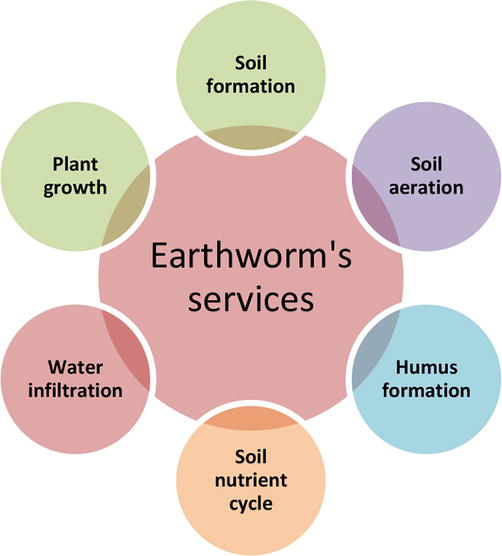
\includegraphics[width=0.4\textwidth]{EW_services.png}
						\caption{Les services écosystémiques rendus par les vers de terre\footnotemark.}\label{fig_wormsservices}
						%legende
					\end{center}
				\end{figure}
			\end{column}
		\end{columns}
		\footnotetext{\textit{Extrait de:} The Earthworms: Charles Darwin’s Ecosystem Engineer, Kumar et al.  (2023).}
	\end{frame}

	\begin{frame}
		\frametitle{\underline{Objectifs:}}
		\textbf{Les méthodes statistiques de Text-mining permettent-elles d’identifier des
		groupes distincts d’articles scientifiques défendant une conception opposée du
		rôle écologique du vers de terre au sein du corpus de texte fourni pour l’analyse ?}
		
		
		\vspace{\baselineskip}
		Pour répondre à cette question de recherche, j'ai procédé en 2 étapes: 
		\begin{enumerate}
				\item Constituer une base de données d'abstracts (courts résumés) d'articles scientifiques \textbf{issus de 4 métaanalyses} différentes du domaine par requêtage d'API et Web-scraping (récupération des données d'un site web grâce à un script) avec Python.
				\item Analyser ces abstracts sous R, par une approche de Text-mining (analyse de données textuelles massives grâce à un script), pour tenter de résoudre cette controverse.
			\end{enumerate}
	\end{frame}

	\section*{Données et scripts}
	\subsection*{Base de données / Scripts} % PBTQ, à remettre dans chaque ss.
	\begin{frame}
		\frametitle{\underline{Base de données:}}
		\begin{columns}
			\begin{column}{0.4\textwidth} % permet diviser la frame en deux colonnes, chacune occupant 50% de l'espace total disponible.
				\begin{enumerate}
					\item Ligne: 1 article / ligne.
					\item La colonne "Abstract" est la plus importante, car elle contient les \textit{textes à analyser}.
				\end{enumerate}
			\end{column}
			\begin{column}{0.6\textwidth}
				\begin{figure}[htb] %le h entre crochet signifie je veux la figure à cet emplacement
					\begin{center} %centrer la figure
						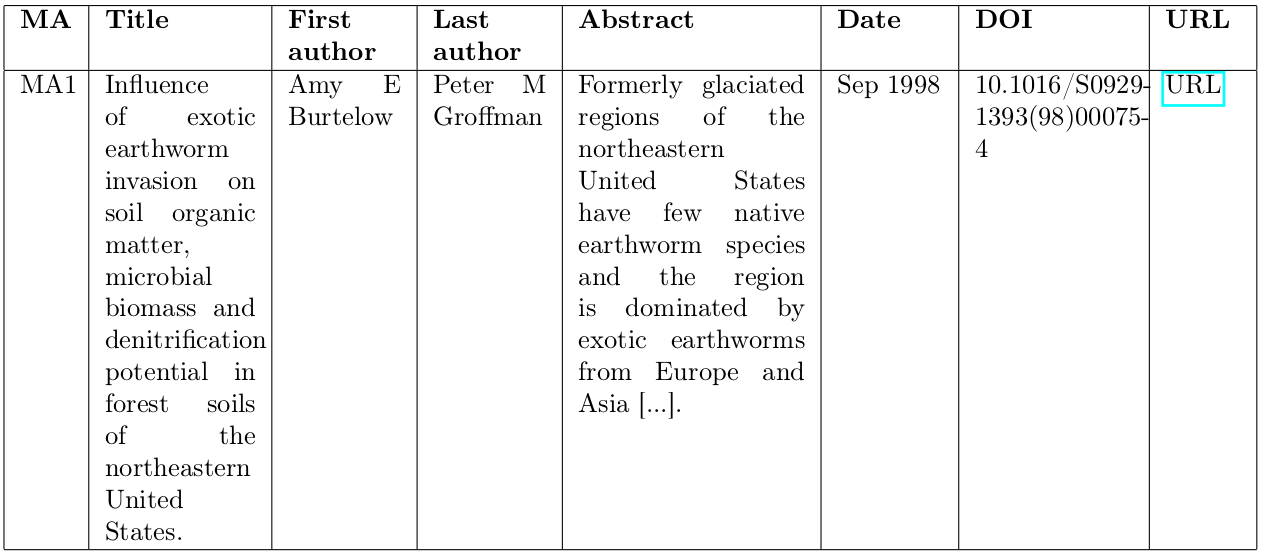
\includegraphics[width=1\textwidth]{screenshotCSV.png}
						\caption{Tableau présentant un exemple de la structure type du fichier CSV issu du Web-scraping et
						employé pour l’analyse. Le fichier originel comprend 168 lignes. Les données manquantes (non représentées ici), sont
						notées "N/A".}\label{fig_exemple_bdd}
						%legende
					\end{center}
				\end{figure}
			\end{column}
		\end{columns}
	\end{frame}

	\begin{frame}
		\frametitle{\underline{Scripts Python et R:}}
		\begin{columns}
			\begin{column}{0.5\textwidth} % permet diviser la frame en deux colonnes, chacune occupant 50% de l'espace total disponible.
				\begin{enumerate}
					\item \textbf{Script Python:} Pour le Web-scraping. \\ \textit{Principaux modules: habanero (Crossref) / ittertools / numpy / pandas / unidecode / ResearchGateScraper2 (module local, incluant re, time, parsel et playwright.sync\_api)}.
					\item \textbf{Script R:} Pour le Text-mining. \\ \textit{Principaux modules: dplyr, ggplot2, ggraph, SnowballC, scales, tidytext.}
				\end{enumerate}
			\end{column}
			\begin{column}{0.5\textwidth}
				\begin{figure}[htb] %le h entre crochet signifie je veux la figure à cet emplacement
					\begin{center} %centrer la figure
						
\includegraphics[width=0.5\textwidth]{image_python_R.png}
						\caption{Le code de Web-scraping a été implémenté en Python, le code de Text-mining en R (R Markdown). \textit{Source de l'image:} https://rstudio.github.io/reticulate/ (image employée à titre illustratif seulement).}\label{fig_python_R}
						%legende
					\end{center}
				\end{figure}
			\end{column}
		\end{columns}
	\end{frame}

	\section*{Calculs de fréquence}
	\subsection*{Courbe de Zipf / Fréquences brutes / Comparaison de fréquences / Approche TF-IDF}

	\begin{frame}
		\frametitle{\underline{Courbe de Zipf:}}
		\begin{columns}
			\begin{column}{0.5\textwidth} % permet diviser la frame en deux colonnes, chacune occupant 50% de l'espace total disponible.
				\begin{enumerate}
					\item La loi de Zipf stipule que dans une collection de données ordonnées par fréquence décroissante, la fréquence d'un élément est inversement proportionnelle à son rang (\textit{mots fréquents : en haut à gauche / mots rares: en bas à droite}).  
					\item La MA3 (\textit{courbe grise}) contient davantage de mots très fréquents que les autres, dont la distribution de mots semble plus proche du modèle linéaire.
				\end{enumerate}
			\end{column}
			\begin{column}{0.5\textwidth}
				\begin{figure}[htb] %le h entre crochet signifie je veux la figure à cet emplacement
					\begin{center} %centrer la figure
						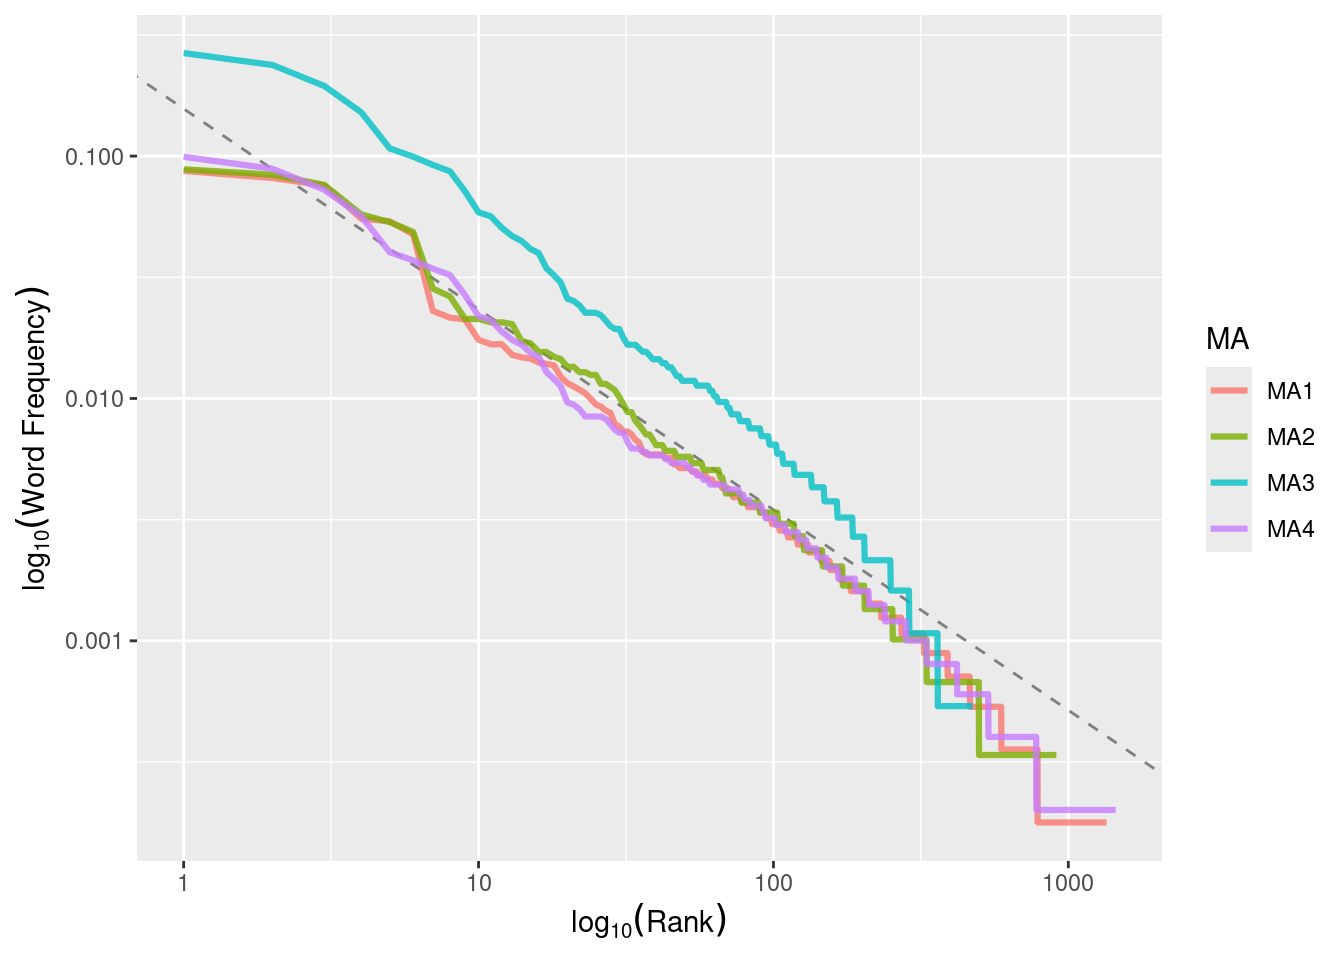
\includegraphics[width=1\textwidth]{curve_zipf.png}
						\caption{Allure de la courbe de Zipf pour les MA1, 2, 3 et 4.La droite en pointillés représente la valeur attendue selon un modèle linéaire sur l’intervalle
						[11,99].}\label{Zipf}
						%legende
					\end{center}
				\end{figure}
			\end{column}
		\end{columns}
		\vspace{\baselineskip}
		Here is some rambling text
	\end{frame}

	\begin{frame}
		\frametitle{\underline{Fréquences brutes:}} 
		\begin{columns}
			\begin{column}{0.5\textwidth} % permet diviser la frame en deux colonnes, chacune occupant 50% de l'espace total disponible.
				\begin{enumerate}
					\item Les trois racines les plus fréquentes dans les articles des quatres métaanalyses confondues sont \textit{earthworm, soil} et \textit{plant}.
					\item Cela semble cohérent avec ce que nous savons des métaanalyses, qui traitent donc bel et bien, toutes trois, du rôle écologique du vers de terre.
				\end{enumerate}
			\end{column}
			\begin{column}{0.5\textwidth}
				\begin{figure}[htb] %le h entre crochet signifie je veux la figure à cet emplacement
					\begin{center} %centrer la figure
						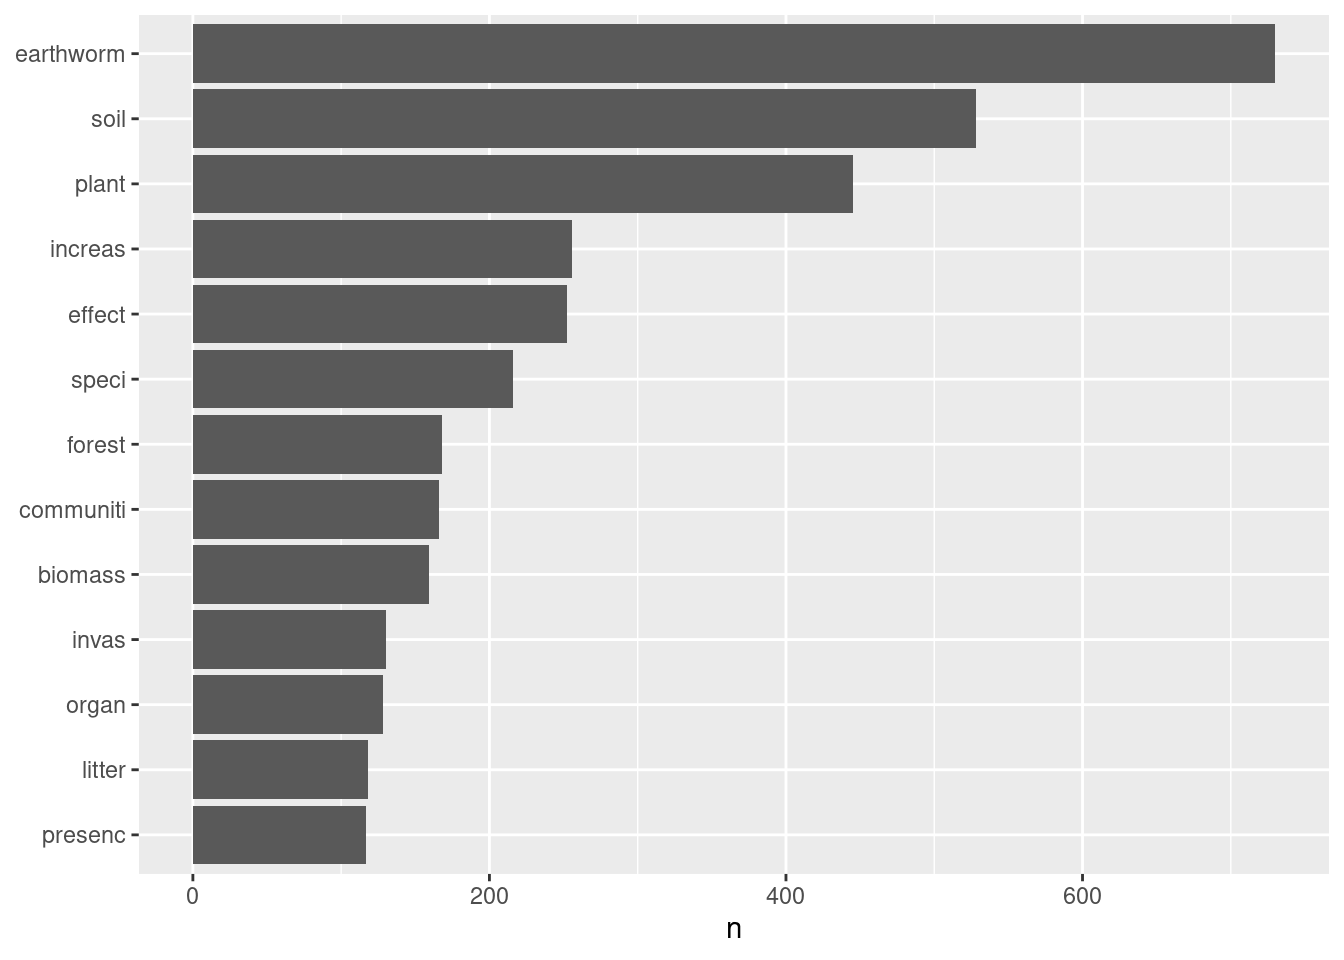
\includegraphics[width=1\textwidth]{freq_all_MA.png}
						\caption{Diagramme à barre représentant les mots les plus fréquents dans l'ensemble des corpus étudiés. Les trois racines les plus fréquentes sont \textit{earthworm, soil} et \textit{plant}.}\label{all_freq}
						%legende
					\end{center}
				\end{figure}
			\end{column}
		\end{columns}
	\end{frame}

	\begin{frame}
		\frametitle{\underline{Comparaison de fréquences:}}
		\begin{columns}
			\begin{column}{0.5\textwidth} % permet diviser la frame en deux colonnes, chacune occupant 50% de l'espace total disponible.
				\begin{enumerate}
					\item List item 1
					\item List item 2
				\end{enumerate}
			\end{column}
			\begin{column}{0.5\textwidth}
				\begin{figure}[htb] %le h entre crochet signifie je veux la figure à cet emplacement
					\begin{center} %centrer la figure
						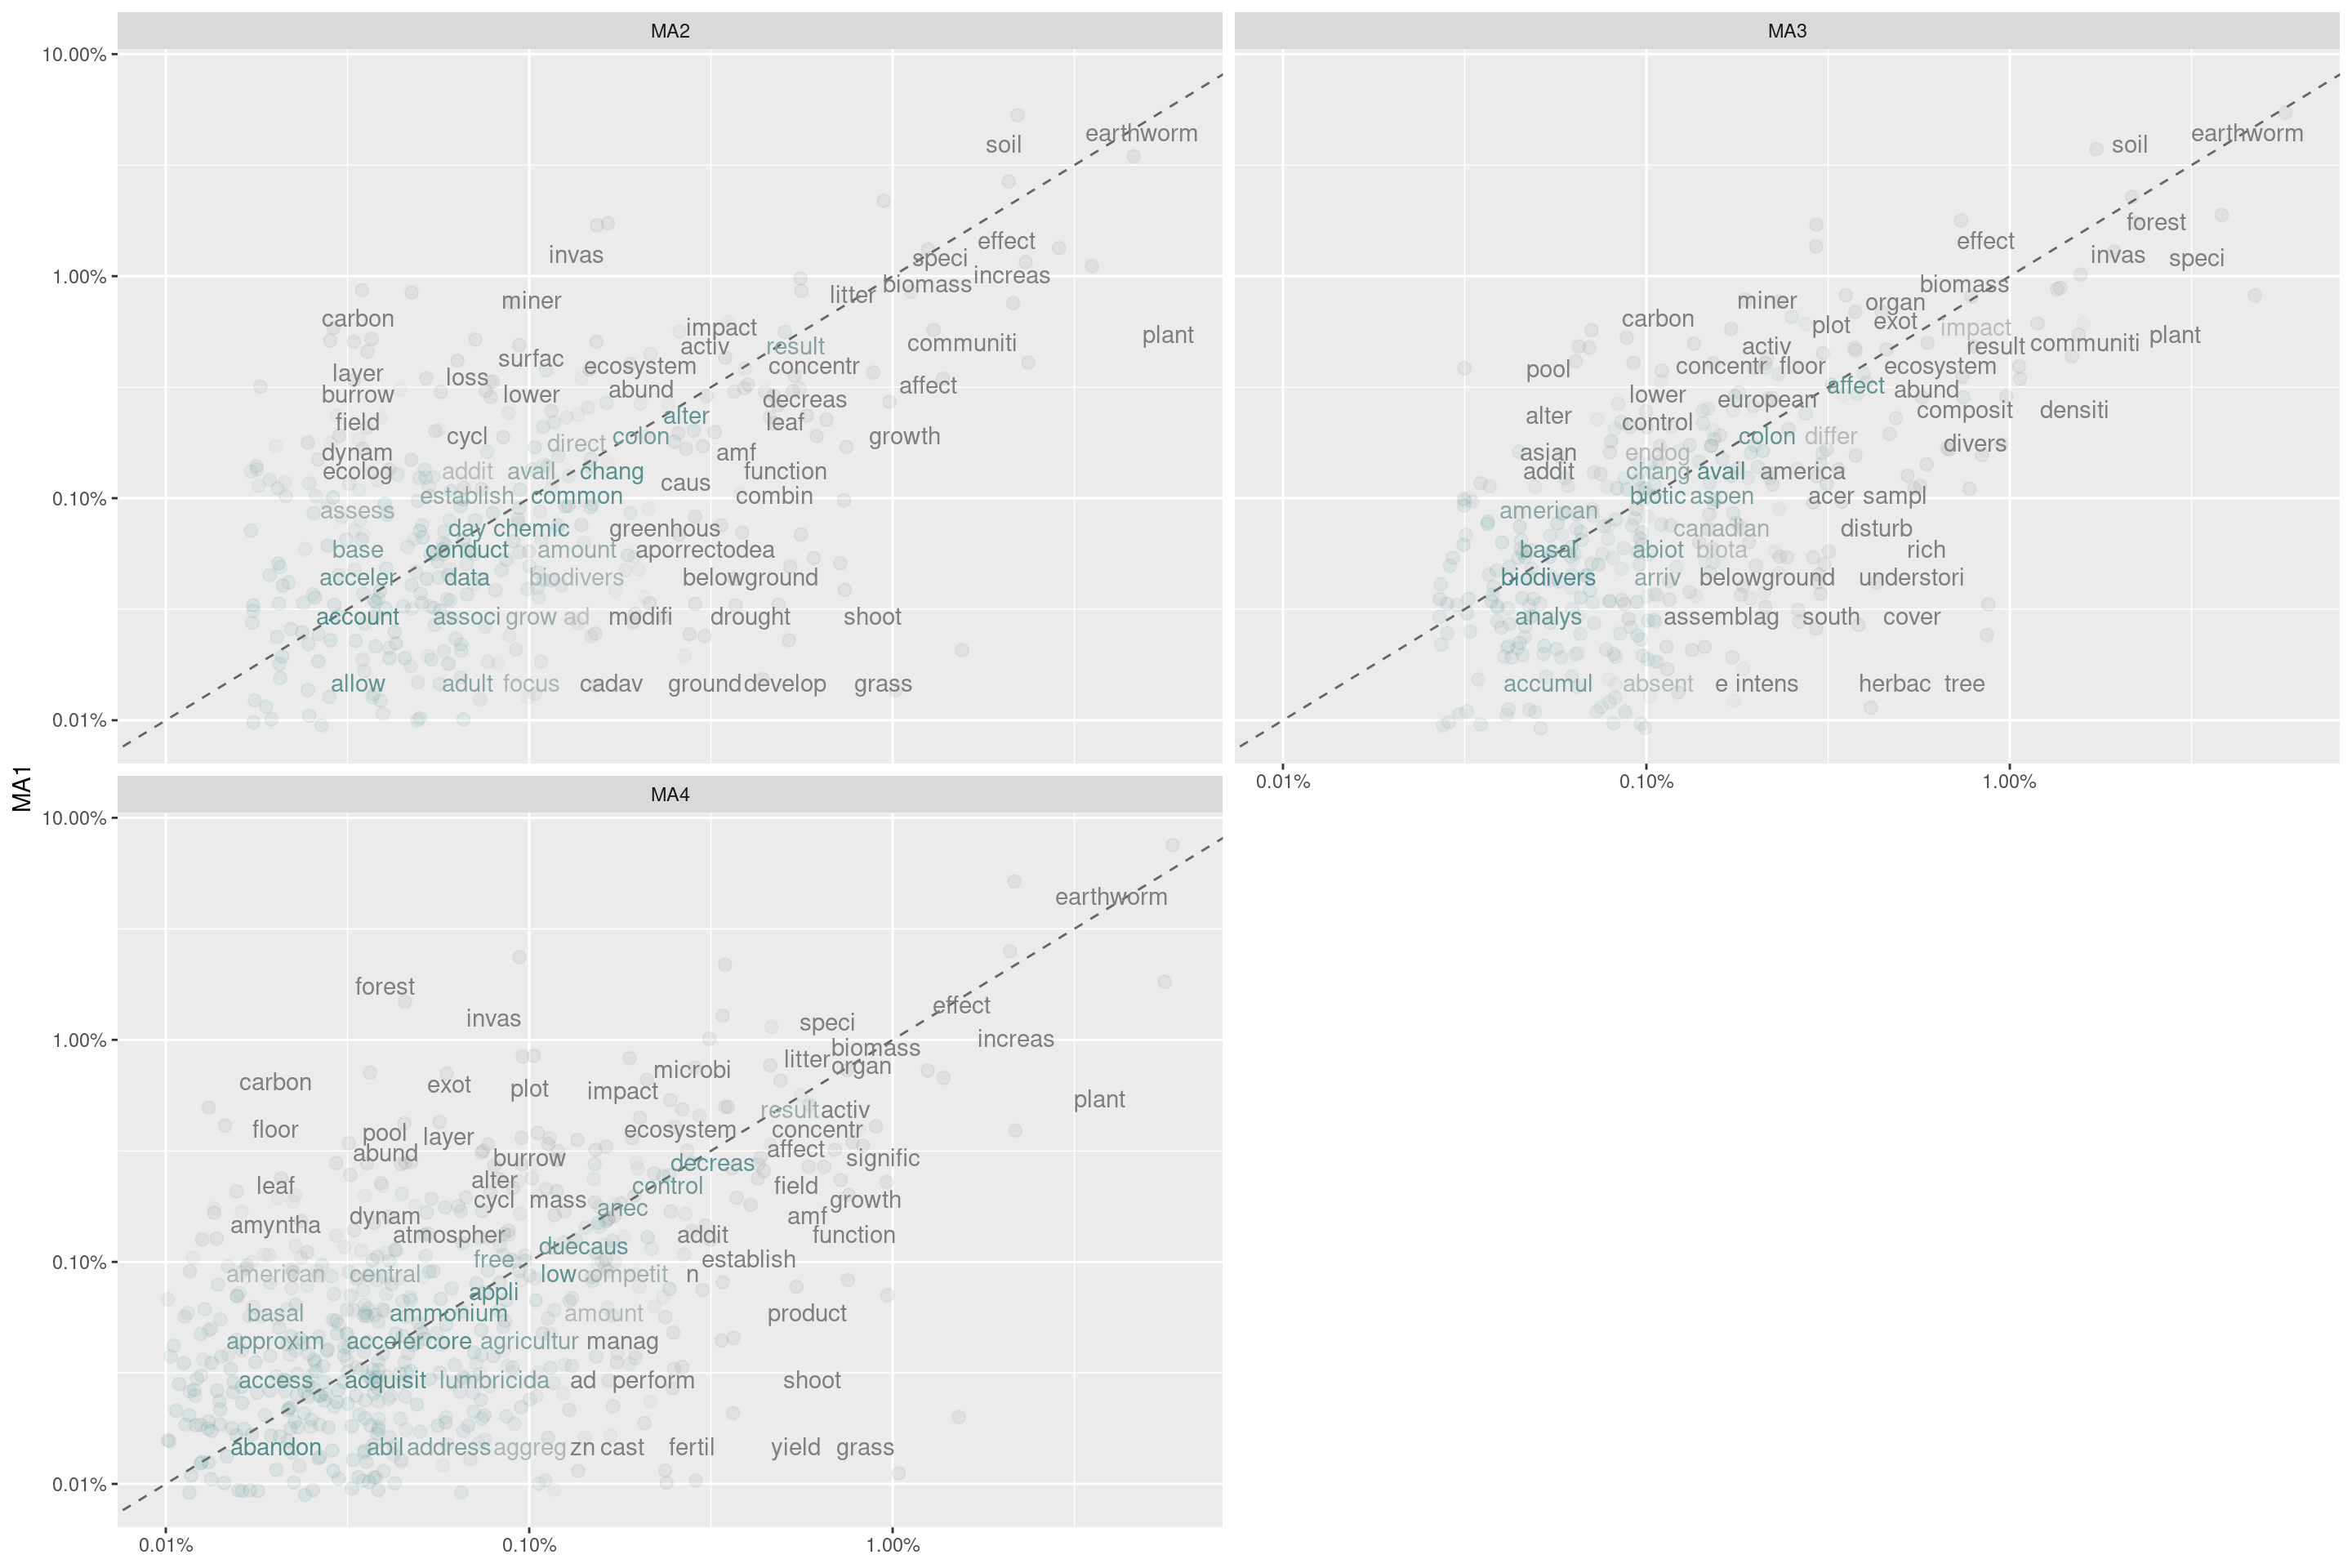
\includegraphics[width=1\textwidth]{scales_graph.png}
						\caption{Log-log scatter plot montrant les corrélations du choix des mots entre les métaanalyses. Les mots sur la ligne grise en pointillés ont une fréquence similaire dans les deux MA comparées.}\label{log_log_sp}
						%legende
					\end{center}
				\end{figure}
			\end{column}
		\end{columns}
		\vspace{\baselineskip}
		Here is some rambling text
	\end{frame}

	\begin{frame}
		\frametitle{\underline{Approche TF-IDF:}}
		Bla bla 
		\begin{columns}
			\begin{column}{0.5\textwidth} % permet diviser la frame en deux colonnes, chacune occupant 50% de l'espace total disponible.
				\begin{enumerate}
					\item List item 1
					\item List item 2
				\end{enumerate}
			\end{column}
			\begin{column}{0.5\textwidth}
				\begin{itemize}
					\item List item 1
					\item List item 2
				\end{itemize}
			\end{column}
		\end{columns}
		\vspace{\baselineskip}
		Here is some rambling text
	\end{frame}

	\section*{Analyse de bigrammes}
	\subsection*{TF-IDF sur les bigrammes / Réseaux de bigrammes}

	\begin{frame}
		\frametitle{\underline{TF-IDF sur les bigrammes:}}
		Bla bla 
		\begin{columns}
			\begin{column}{0.5\textwidth} % permet diviser la frame en deux colonnes, chacune occupant 50% de l'espace total disponible.
				\begin{enumerate}
					\item List item 1
					\item List item 2
				\end{enumerate}
			\end{column}
			\begin{column}{0.5\textwidth}
				\begin{itemize}
					\item List item 1
					\item List item 2
				\end{itemize}
			\end{column}
		\end{columns}
		\vspace{\baselineskip}
		Here is some rambling text
	\end{frame}

	\begin{frame}
		\frametitle{\underline{Réseaux de bigrammes:}}
		Bla bla 
		\begin{columns}
			\begin{column}{0.5\textwidth} % permet diviser la frame en deux colonnes, chacune occupant 50% de l'espace total disponible.
				\begin{enumerate}
					\item List item 1
					\item List item 2
				\end{enumerate}
			\end{column}
			\begin{column}{0.5\textwidth}
				\begin{itemize}
					\item List item 1
					\item List item 2
				\end{itemize}
			\end{column}
		\end{columns}
		\vspace{\baselineskip}
		Here is some rambling text
	\end{frame}

	\section*{Analyse de sentiment}
	\subsection*{Wordclouds / Mots simples / Bigrammes}

	\begin{frame}
		\frametitle{\underline{Wordclouds:}}
		Bla bla 
		\begin{columns}
			\begin{column}{0.5\textwidth} % permet diviser la frame en deux colonnes, chacune occupant 50% de l'espace total disponible.
				\begin{enumerate}
					\item List item 1
					\item List item 2
				\end{enumerate}
			\end{column}
			\begin{column}{0.5\textwidth}
				\begin{itemize}
					\item List item 1
					\item List item 2
				\end{itemize}
			\end{column}
		\end{columns}
		\vspace{\baselineskip}
		Here is some rambling text
	\end{frame}

	\begin{frame}
		\frametitle{\underline{Mots simples:}}
		Bla bla 
		\begin{columns}
			\begin{column}{0.5\textwidth} % permet diviser la frame en deux colonnes, chacune occupant 50% de l'espace total disponible.
				\begin{enumerate}
					\item List item 1
					\item List item 2
				\end{enumerate}
			\end{column}
			\begin{column}{0.5\textwidth}
				\begin{itemize}
					\item List item 1
					\item List item 2
				\end{itemize}
			\end{column}
		\end{columns}
		\vspace{\baselineskip}
		Here is some rambling text
	\end{frame}

	\begin{frame}
		\frametitle{\underline{Bigrammes:}}
		Bla bla 
		\begin{columns}
			\begin{column}{0.5\textwidth} % permet diviser la frame en deux colonnes, chacune occupant 50% de l'espace total disponible.
				\begin{enumerate}
					\item List item 1
					\item List item 2
				\end{enumerate}
			\end{column}
			\begin{column}{0.5\textwidth}
				\begin{itemize}
					\item List item 1
					\item List item 2
				\end{itemize}
			\end{column}
		\end{columns}
		\vspace{\baselineskip}
		Here is some rambling text
	\end{frame}

	\section*{Conclusion}
	\subsection*{Rappel des résultats et perspectives}

	\begin{frame}
		Bla bla 
		\begin{columns}
			\begin{column}{0.5\textwidth} % permet diviser la frame en deux colonnes, chacune occupant 50% de l'espace total disponible.
				\begin{enumerate}
					\item List item 1
					\item List item 2
				\end{enumerate}
			\end{column}
			\begin{column}{0.5\textwidth}
				blabla
			\end{column}
		\end{columns}
		\vspace{\baselineskip}
		Here is some rambling text
	\end{frame}
\end{document}

















% 15 DIAPOS EN M1 BIMS.

% MANUEL:

% FAIRE UNE FRAME COUPÉE EN 2 AU MILIEU:
%  	\begin{frame}
% 	Bla bla 
% 	\begin{columns}
% 		\begin{column}{0.5\textwidth} % permet diviser la frame en deux colonnes, chacune occupant 50% de l'espace total disponible.
% 			\begin{enumerate}
% 				\item List item 1
% 				\item List item 2
% 			\end{enumerate}
% 		\end{column}
% 		\begin{column}{0.5\textwidth}
% 			\begin{itemize}
% 				\item List item 1
% 				\item List item 2
% 			\end{itemize}
% 		\end{column}
% 	\end{columns}
% 	\vspace{\baselineskip}
	
% 	Here is some rambling text

% \end{frame}

% CAPTION:
% Ne supporte pas le retour à la ligne "\\".